% This file is meant to be included in another 
\documentclass{article}
\usepackage{epsfig}
\begin{document}

\section{\tt{CrossCorr()}}

\subsection{Purpose}

Computes the cross-correlation statistic for two interferometers.  

\subsection{Synopsis}

\begin{verbatim}
void CrossCorr (Status*, REAL4*, CCIn*);

typedef struct tagCCIn {            /* input structure        */
       REAL4TimeSeries  *g1;        /* output of detector 1   */
       REAL4TimeSeries  *g2;        /* output of detector 2   */
       REAL4Vector      *QmaxTilde; /* optimized kernel       */
       INT2             plan;       /* 1 -> estimate plan ... */
                                    /* otherwise measure plan */
} CCIn;
\end{verbatim}

\subsection{Description}

{\tt CrossCorr()\/} will compute
the cross correlation statistic $\sl{Y}_{\mathrm{max}}({ \bf{g} }) $
%
\begin{equation}
\label{ymax}
\sl{Y}_{\mathrm{max}}({ \bf{g} })=\
\frac{1}{2N-1}\
\sum_{j=-(N-1)}^{N-1}\
\widetilde{\bar{g}}_{1}[j]^*\
\widetilde{Q}_{\mathrm{max}}[j]\
\widetilde{\bar{g}}_{2}[j],
\end{equation}
%
where $Q_{\rm{max}}$ is the optimized 
kernel, $g_i$ is the dimensionless strain output of the $i^{\rm{th}}$ detector, and $N$ is the number of
samples in the $g_i$. The tilde indicates discrete Fourier transform, $^{*}$ indicates complex conjugation, 
and the overbar indicates zero-padding:
%
\begin{equation}\nonumber
\bar{g}_{i}[j]=\
\left\{ \begin{array}{cl}
	g_{i}[j]  &    j = 0, 1, \cdots, N-1 \\
	0         &    j = -1, -2, \cdots, -(N-1)
	\end{array}
\right.
\end{equation}
%
and $\widetilde{Q}_{\mathrm{max}}[j]$.  Each of the detector outputs must be 
{\tt REAL4TimeSeries} and the kernel must be a {\tt REAL4Vector}.

We assume $Q_\mathrm{max}[j]$ is both real and even. Therefore we must also have a real and even
$\widetilde{Q}_\mathrm{max}[j]$.  
This means that the sum in equation \ref{ymax} for $j<0$
is simply the complex conjugate of the sum for $j>0$.
Thus it is more efficient to compute
$Y_\mathrm{max}$ in the form:
\begin{equation}\label{shortcut}
\sl{Y}_{\mathrm{max}}({ \bf{g} })=\
\frac{1}{2N-1}\
\left(
\widetilde{\bar{g}}_{1}[0]^*\
\widetilde{Q}_{\mathrm{max}}[0]\
\widetilde{\bar{g}}_{2}[0]+\
2\sum_{j=1}^{N-1}\
{\mathrm{Re}} \left\{
\widetilde{\bar{g}}_{1}[j]^*\
\widetilde{Q}_{\mathrm{max}}[j]\
\widetilde{\bar{g}}_{2}[j]
\right\}
\right)
\end{equation}

\subsection{Operationg instructions}

The use of {\tt CrossCorr()} is sketched below.

\begin{verbatim}
Status          status;
CCIn            in;
REAL4           out;

/* this is where you fill the input structure */

/* compute the cross-correlation statistic */
CrossCorr(&status, &out, &in); 
\end{verbatim}

\subsubsection{Arguments}

\begin{itemize}
\item
{\tt status\/} is a universal status structure.
Its contents are initially assigned by {\tt InitStatus()\/} and then
set by {\tt CrossCorr()\/} on return.
Non-zero status codes indicate an error condition as specified in
Table~\ref{t:errors}
\item
{\tt in\/} is the input structure containing the single precision 
time domain output from the two detectors, the single precision 
optimized kernel, and an integer used to specify the type of FFT plan to 
use (see options).
\item
{\tt out\/} is a single precision real number for output. Although memory 
must be allocated for {\tt out}, no particular initial value is necessary.
\end{itemize}

\subsubsection{Options}

The user can choose whether to use the {\tt MeasureFwdRealFFTPlan} or \\
{\tt EstimateFwdRealFFTPlan} for the FFTs.  The default plan is 
{\tt MeasureFwdRealFFTPlan}.  However, if {\tt in.plan == 1} 
we use {\tt EstimateFwdRealFFTPlan}.


\subsubsection{Error conditions}

{\tt CrossCorr()\/} sets the universal status structure on return.
Non-zero status codes indicate an error condition.
Error conditions are described in Table~\ref{t:errors}.

\begin{table}
\hskip -.75cm
\begin{tabular}{|r|l|l|}\hline
status	& status			& Description					\\
code	& description			& \\\hline
EIN	& {\tt \&in == NULL}		& Pointer to input structure must be non-NULL	\\
EOUT	& {\tt \&out == NULL}		& Pointer to output value must be non-NULL	\\
ENULL   & {\tt in.g1->data == NULL}	& The pointers to the detector output vectors	\\
	& {\tt || in.g2->data == NULL}	& must be non-NULL				\\
ESIZE1	& {\tt in.g1->data->length}	& Detector output vectors must have equal	\\
	& {\tt != in.g2->data->length}	& length					\\
ESIZE2	& {\tt in.QmaxTilde->length}	& Kernel vector and detector output vectors	\\
	& {\tt != in.g1->data->length}	& must have equal length			\\
\hline
\end{tabular}
\caption{Error conditions for {\tt CrossCorr()\/}}
\label{t:errors}
\end{table}

\subsection{Algorithms}

The cross-correlation statistic is computed by straight forward application of equation \ref{shortcut}.  
We zero-pad the detector outputs, apply the discrete Fourier transform, and then sum. 

\subsection{Accuracy}

The cross-correlation statistic is calculated to single precision.

\subsection{Tests}

The testing program {\tt CrossCorrTest} tests all the error checking devices.
It also compares the results of three test calculatoins 
with expected values.  The tests differ only in choice of kernel. 
The sample detector outputs and the three different kernels which are used in the tests 
are shown in figure \ref{test}.
\begin{figure}
\begin{center}
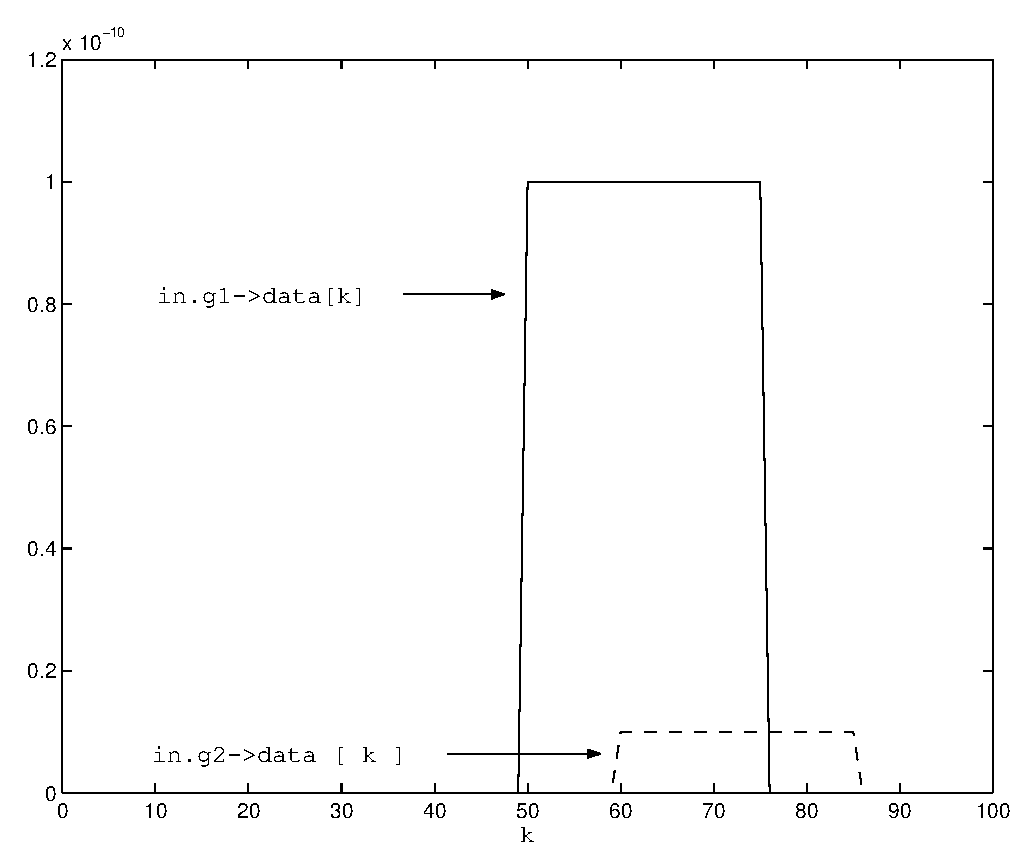
\includegraphics[width=5cm]{data}
\includegraphics[width=5cm]{kernel1}
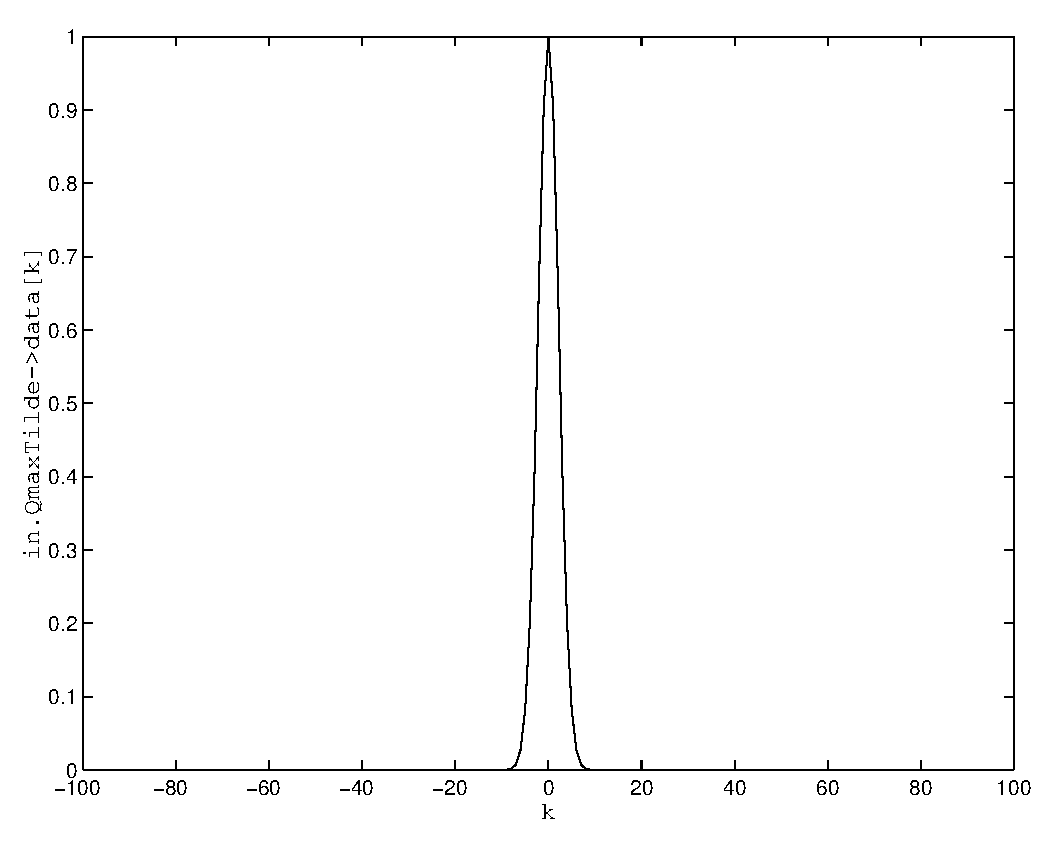
\includegraphics[width=5cm]{kernel2}
\includegraphics[width=5cm]{kernel3}
%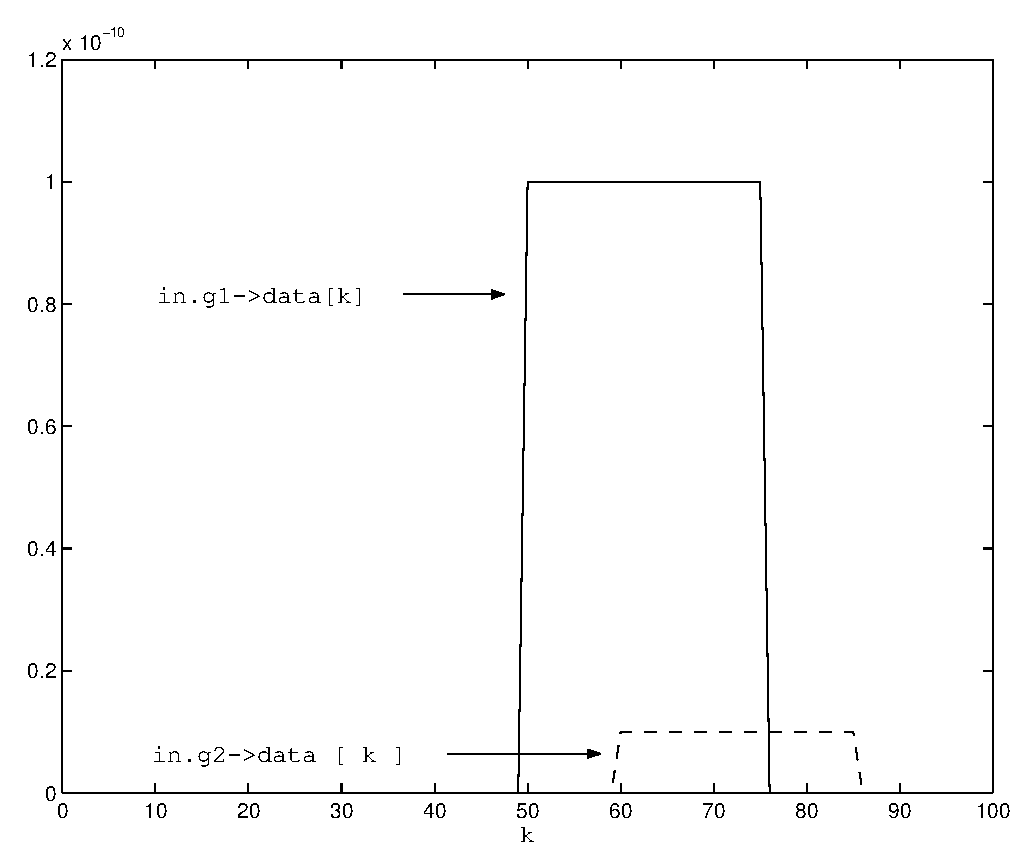
\epsfig{file=data.eps,width=5cm}
%\epsfig{file=kernel1.eps,width=5cm}
%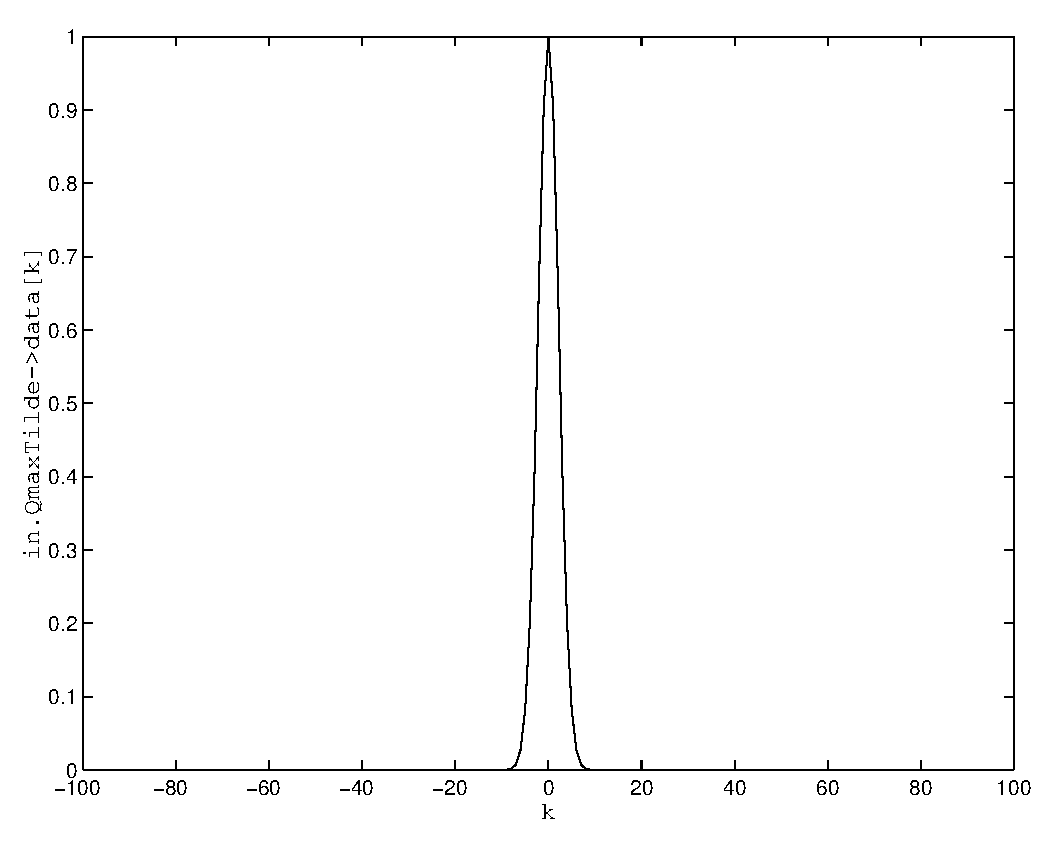
\epsfig{file=kernel2.eps,width=5cm}
%\epsfig{file=kernel3.eps,width=5cm}
\end{center}
\caption{sample data and kernels uesd for tests}%
\label{test}%
\end{figure}

\subsection{Uses}

We use the following LAL functions:

\begin{itemize}
\item{\tt InitStatus()\/}
\item{\tt SCreateVector()\/}
\item{\tt SDestroyVector()\/}
\item{\tt CCreateVector()\/}
\item{\tt CDestroyVector()\/}
\item{\tt MeasureFwdRealFFTPlan()\/}
\item{\tt EstimateFwdRealFFTPlan()\/}
\item{\tt FwdRealFFT()\/}
\item{\tt DestroyRealFFTPlan()\/}
\end{itemize}

\subsection{Notes}

None 

\begin{thebibliography}{0}

\bibitem{samjoe}
L.S. Finn and J.D. Romano, \emph{Detecting stochastic gravitational waves: Performance of 
maximum-likelihood and cross-correlation statistics}, in preperation, (1999)

\end{thebibliography}

\end{document}
